%%%%%%%%%%%%%%%%%%%%%%%%%%%%%%%%%%%%%%%%%%%%%%%%%%%%%%%%%%%
% EPFL report package, main thesis file
% Goal: provide formatting for theses and project reports
% Author: Mathias Payer <mathias.payer@epfl.ch>
%
% This work may be distributed and/or modified under the
% conditions of the LaTeX Project Public License, either version 1.3
% of this license or (at your option) any later version.
% The latest version of this license is in
%   http://www.latex-project.org/lppl.txt
%
%%%%%%%%%%%%%%%%%%%%%%%%%%%%%%%%%%%%%%%%%%%%%%%%%%%%%%%%%%%
\documentclass[a4paper,11pt,oneside]{report}
% Options: MScThesis, BScThesis, MScProject, BScProject
\usepackage[MScProject,lablogo]{EPFLreport}
\usepackage{graphicx}
\usepackage{listings}
\graphicspath{ {./figures/} }
\usepackage{xspace}

\title{Semester project on Fuzzing Trusted Execution Environments on COTS Android Devices}
\author{Leonardo Pennino}
\supervisor{Marcel Busch}
\adviser{Prof. Dr. sc. ETH Mathias Payer}
%\coadviser{Second Adviser}

\newcommand{\sysname}{TEEzz\xspace}

\begin{document}
\maketitle
\makeacks

\begin{abstract}
  The \sysname \cite{TEEzz} tool designed by Dr. Marcel Busch enables effective fuzzing of
Trusted Environment by an automatic infer of the data and value dependency
obtained by looking at the interactions of the TA.
The goal of the project is to continue the implementation by building and all
the required parts for the Fuzzer to work. The main work was focused on fixing
and improving the existing Client Application Library Identification (CAID)
tool by enabling multithreaded computation, creating drivers for Trusted
Application in order to trigger interactions with the TEE, improving the build system of the seed recorder and generate working recorders
for the device Hikey620.
\end{abstract}

\maketoc

\chapter{Introduction}

This project's aim is to continue the development of the TEEzz tool via rewriting
a part of the source code to give it a better structure a software engineering
point of view, adding more test cases and supported libraries, improving performance and making the infrastructure testable
and reusable by other researchers.
\paragraph{TEEzz-CAID}
The tool TEEzz-CAID which originally was working only on Android Devices of
some specific vendors was rewritten to support any vendor by building and
injecting missing binaries on the phone which are essential for the tool,
furthermore the program was sped up by dividing its computation in multiple
threads, and restructured for easier understanding from other researchers.
\paragraph{Writing drivers for closed sourced client applications}
The repository contains an example driver for Mlipay, which is a Xiaomi library
that handles payments on smartphones. The driver is currently able to call one function
of the TA.
\paragraph{Writing drivers using Java Reflection}
The project contains drivers for "Gatekeeper" and "Keystore" which using android
binder mechanisms, allow us to call into the Client Application by using Java
Methods. All functionalities of Keystore and Gatekeeper were implemented in the driver.
\paragraph{Seed Recording}
The seed recording was made into a docker container able to automatically
download the android code, compile required libraries, and set up all the
required objects for the recorder to work with. In particular, it was automated
the generation of header files from Android's HIDL files and the js code required
by frida for the test device \emph{Hikey620}.
\paragraph{Resources}
The project is divided in 3 different repositories:
\begin{itemize}
  \item \href{https://github.com/HexHive/teezz-caid}{TEEzz-CAID}
  \item \href{https://github.com/HexHive/teezz-ca-driver}{TEEzz-ca-driver}
  \item \href{https://github.com/HexHive/teezz-introspection}{Teezz-introspection}
\end{itemize}

%%%%%%%%%%%%%%%%%%%%%%
%%%%%%%%%%%%%%%%%%%%
\chapter{Background}
%%%%%%%%%%%%%%%%%%%%

Explain how android Binder works, how trusted applications communicate and
the goal of teezz
Communications with the main ta
library are usually handled with a central library (as libteec.so).
%%%%%%%%%%%%%%%%%%%
\chapter{Library Identification}
%%%%%%%%%%%%%%%%%%%
The first goal of the project is to provide a mean to detect which Android
Applications or libraries are accessing the Trusted Execution Enviroment.
To achieve this goal the tool "teezz-caid" is able to
scan an android device and look for every app or library that is directly or
indirectly calling communicating with the TA. The program requires as input
the \emph{main} CA library for that specific device e.g.:\emph{libteec.so}.
The program will then build a graph where on its vertexes we find all the
libraries and consumers that eventually call into the ta which is the root node.
The process is divided in three parts:
Downloading binaries, Disassembling and Finding Dependencies.
\section{Downloading binaries}
The first part of the process relies in getting all executables, libraries
and VDexs from the device. In order to do so we spawn a shell and we execute
\emph{file} for each one of them. The first problem faced was that many vendors
do not include all required \emph{unix binaries} which are needed by the program
such as \emph{file} or \emph{find}. To solve this problem we have statically
compiled those utilities that will be injected into the device where needed.
Another issue is that pulling large amounts of files from android phones takes
time, to solve this we divide the pulling in more threads to speed up the
process.

\section{Disassembling}
Once the program downloads the required files, we have two different categories
of files and each will be treated differently: \textbf{ELF files},
and \textbf{VDexs}. For ELF files \emph{readelf} is used to get all the libraries
needed by the executable. It will also list libraries loaded with \emph{dlopen}
by specifically looking for the \emph{dlopen} or
\emph{hw \textunderscore get\textunderscore module} symbols.
\emph{VDexs} files instead are firstly extracted using vdexExtractor, then
decompiled using jadx. Once that is done a process similar to ELFs is followed,
in particular we look for \emph{System.LoadLibrary} to check which libraries
it is using.
\section{Finding Dependencies}
At the end of the before mentioned process, a list of Vdexs and Elfs is obtained, each one with
their own dependencies. The program starts by putting the main CA library given
as input on a stack, then it will scan the built list for every file that has
that library as a dependency. Every match is put on the stack and the previous
item is popped, then recursively repeats the
process until no items remain on the stack. At the end we obtain
a graph with all the found libraries and applications. Below is an image
of a graph obtained for the Nexus 5X.
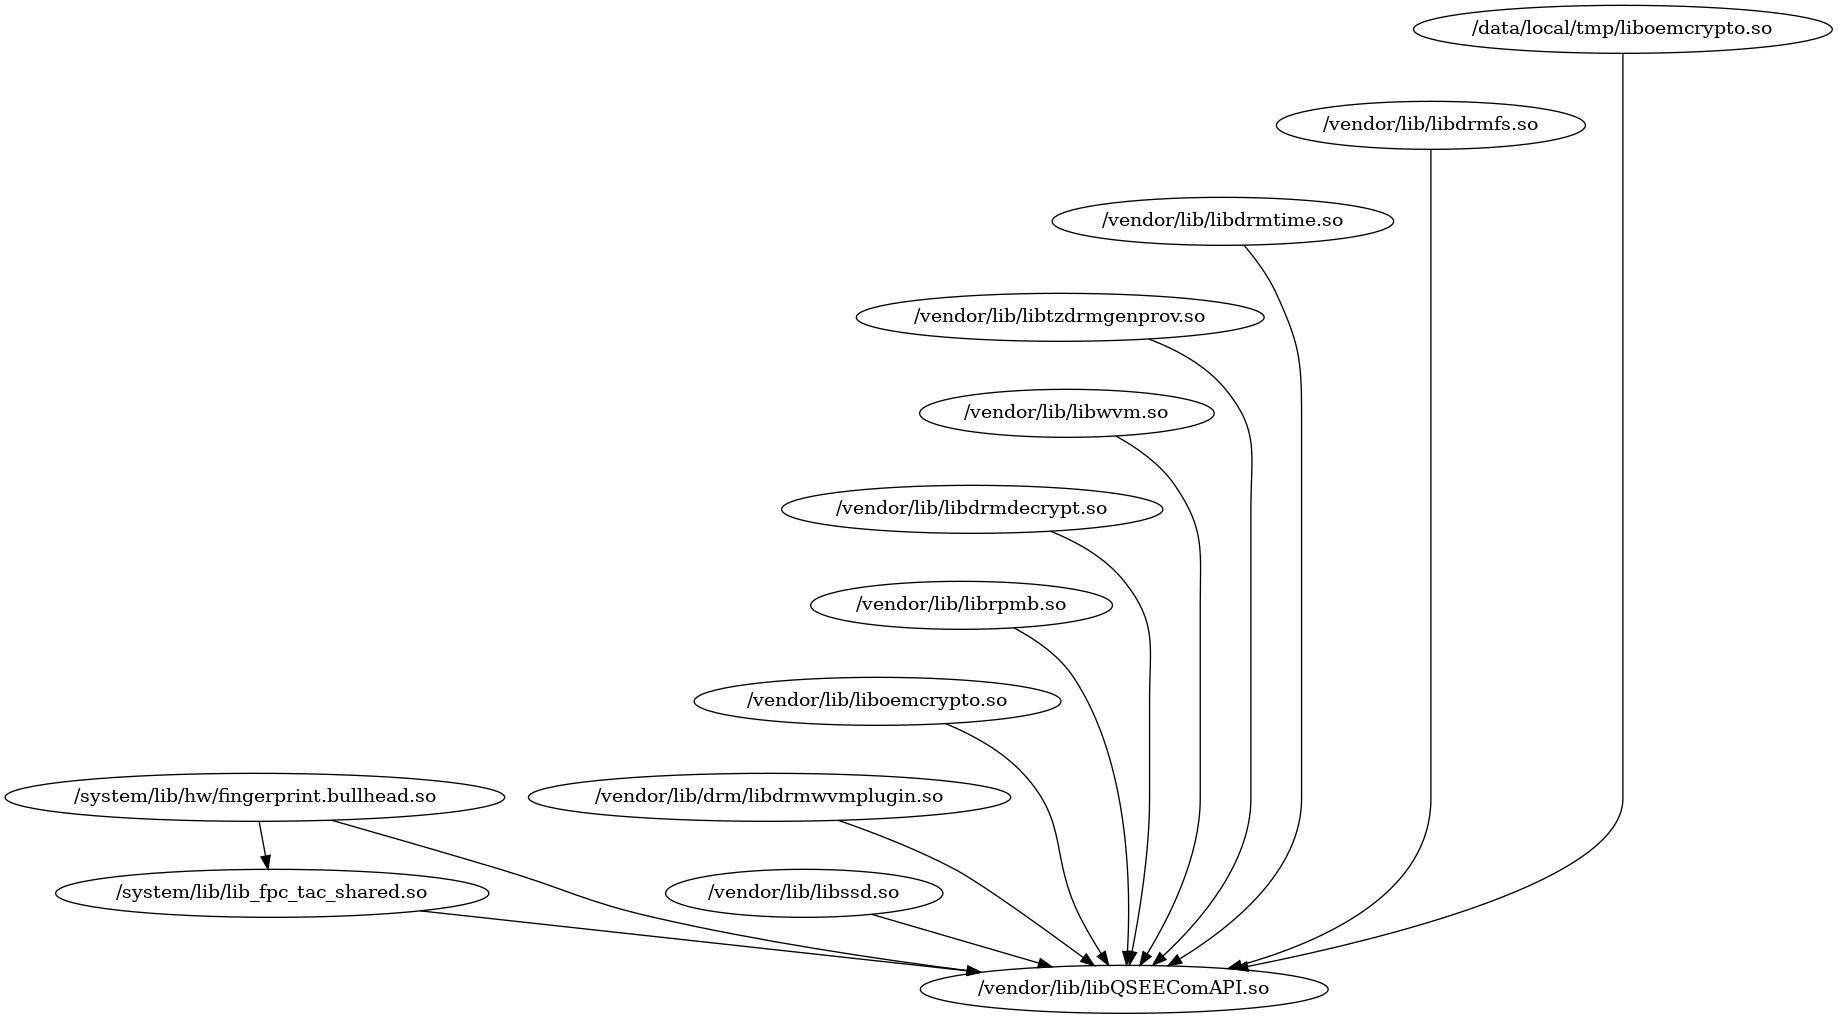
\includegraphics[width=16cm, height=20cm]{figures/nexus5x.png}
%%%%%%%%%%%%%%%%
\chapter{Triggering interactions with the TA: Drivers}
%%%%%%%%%%%%%%%%
After the discovery of the targets, before talking about the fuzzing we have to
first find a way for triggering TA interactions that \sysname relies on for the
data and state infering. Interaction with the TAs can be achieved in two ways:
By manual interaction with the device, or automatically via calling a function
of a Client Application.
\section{Manual Interaction}
Manual interactions with the Trusted Execution Environment happen when
we change things that should be handled by the TEE such as a lockscreen code on an android phone, gatekeeper will trigger a request
to the ta in order to submit and approve the changes. Doing this effort
manually each time requires a lot of time and makes our fuzzing very inefficient.
The first approach was to emulate touches on the android phone using a
program that I designed to trigger the touches as fast as possible.
This solution was fast to implement and correctly working however it
took around 3 minutes for some specific interactions.
Certain android devices such as Huawei in order to
remove the lockscreen code, needed to trigger a particular interaction in the
\emph{Gatekeeper}, require 5 wrong tries, with 30 seconds delay between
each other, thus the whole process took 3 minutes each time.
\section{Interactions using Java Reflection}
Seeing these downfalls, we opted
for another path. We found a way to trigger interactions using Java
Reflection. By exploiting the way Android Binder Mechanism and Android HIDL
Java, we were able to call native libraries code via Java. We first build a
java program which hooks into Android Java classes such as \emph{Gatekeeper}
via \textbf{Class.forName}, then we can trigger methods or create objects.
After having built our java file we \textbf{dex} it and inject into our test device and
run it via \emph{app\textunderscore process}. This approach does not have the
drawbacks of
the one discussed before, however not every Client Application has a java
callable interface, hence why this approach cannot be used in all scenarios.
\begin{lstlisting}[language=Java, caption="Example driver for Keystore"]
public KeystoreClient() {
      Class IKeystoreService = Class.forName(
      "android.security.IKeystoreService");
      Class stub = IKeystoreService.getDeclaredClasses()[0];
      Method mAsInterface = stub.getDeclaredMethods()[0];
      //Final object able to call binder
      oKeystoreService = mAsInterface.invoke(null, getKeystoreBinder());
      //now we can access the methods
      mReset = oKeystoreService.getClass().getDeclaredMethod("reset");
      mGet = oKeystoreService.getClass().getDeclaredMethod("get", String.class, int.class);
      // we can call methods like this
      mGet.invoke(oKeystoreService,...params);
    }
\end{lstlisting}
\section{Interaction with custom C/C++ drivers}
For example Xiaomi's \emph{mlipay} library
which is used for payments, due to it not having a Java HIDL interface, requires the developing of a C++ driver  which is
able to construct the MLIPAY object and call into its functions. In order to
build such a driver, first we have to reverse engineer the library to
understand its functionalities and how it works, then we create an handle and
attach it using \emph{dlopen}.
We have only managed to write a driver for one of MLIPAY's functions as it is
very time consuming to reverse ARM64 android C++ applications.
\begin{lstlisting}[language=C++, caption= Example driver for mlipay]
int main(int argc, char **argv) {
  void *handle = dlopen("libmlipay.so", RTLD_NOW | RTLD_GLOBAL);
  if (handle == NULL) {
    printf("Error opening handle to libmlipay.so");
    return -1;
  }
  void *(*fn)(void) = NULL;
  void *(*constructor)(void) = NULL;
  void *(*get_key_version)(void) = NULL;
  printf("Created handle \n");
  *(void **)(&fn) = dlsym(handle, "HIDL_FETCH_IMlipayService");
  if (fn != NULL) {
    printf("Calling fn\n");
    void **obj = (void **)(*fn)();
    void **vtable = (void **)*obj;
    *(void **)(&constructor) = (void **)*(vtable);
    *(void **)(&get_key_version) = (void **)*(vtable + 0xe);
    //The address above was obtained via reverse engineering
    (*get_key_version)(); // Calling our target function
  }
}
\end{lstlisting}

%%%%%%%%%%%%%%%%%%%%%%%%

%%%%%%%%%%%%%%%%%%%%
\chapter{Seed Recording}
%%%%%%%%%%%%%%%%%%%%
The last part of the project focused on improving and making the seed
recorder portable and easily reproducible and adaptable to various devices.
The seed recorder is the part of the project that is
responsible to create type aware seeds for the fuzzer.
The recording works at different abstraction levels:
\textbf{IOCTL} and the \textbf{Hardware Abstraction Layer}.
It uses Frida to dinamycally instrument code on the target device to execute arbitrary code allowing the inspection and dumping of the memory.
IOCTL is the lowest abstraction layer, it contains no
type definitions, only raw bytes are sent. For this
layer we just need to hook into the \emph{ioctl} system
call and dump the data sent.
The HAL layer is just above the IOCTL and this contains struct definitions, types and value dependencies.
The seeds that need to be generated from HAL and IOCTL are very different. More work is needed for the HAL to correctly identify the data that the
application passes to the TEE.
The seed recorder consists of the following parts: the \textbf{Interceptor}, \textbf{Generator}, \textbf{FridaDumper}, \textbf{HalDumper} and \textbf{DualRecorder}.
\section{Interceptor}
The role of the interceptor is to attach the frida debugger to the function calls we want to look into.
The interceptor takes as parameter a json file describing
the interface's functions and how to locate them, either via symbols if the binary is non stripped or by offset.
It can either attach by symbol name or function offset.
After attaching to a function it automatically dumps the incoming and outgoing parameters.
\label{sec:Gendumper}
\section{Gendumper}
The gendumper takes as input a C/C++ file and a struct or class and dumps the js code which will be then used by frida, with type and state awareness. In order to correctly parse the input file it makes use of clang to build an
AST, which it explores to find the definition for each type and function of the input symbol. To work as
expected, it requires all C / C++ headers that the input file uses. To make the software portable and readaptable, the download and compilation of required libraries has to be automated. The docker container included in the seed recorder contains \emph{Makefiles} for different devices that automatically download and compile the needed libraries from the AOSP and generate the header files required by the gendumper.
\section{FridaDumper}
The FridaDumper instruments the Client Application in order to hook into \emph{ioctl} and dump the data flow.
\section{HalDumper}
The HalDumper takes as input the javascript files generated by the GenDumper and a service to hook into.
It then attaches frida and instruments the binary to
dump function calls, incoming and outgoing parameters for each function contained in the javascript file.
\section{Dual Recorder}
The dual recorder is the final step of the project, it combines both the HalDumper and the Frida Dumper into one unique program which is able to generate both seeds that will then be used by the fuzzer.

\begin{lstlisting}[language=bash , caption=Example of seeds recorded for Keystore on HIKEY620]

exportKey_10000/onenter:
appData
clientId
exportFormat
keyBlob

exportKey_10000/onleave:
appData
clientId
exportFormat
keyBlob

finish_1000/onenter:
inParams
input
operationHandle
signature

finish_1000/onleave:
inParams
input
operationHandle
signature

importKey_13345/onenter:
keyData
keyFormat
params

importKey_13345/onleave:
keyData
keyFormat
params

update_15005/onenter:
inParams
input
operationHandle

update_15005/onleave:
inParams
input
operationHandle

\end{lstlisting}
\chapter{Challenges}
During this project many challenges had to be faced, I will try to give a brief summary of them in chronological order.
\section{On writing handles for C++ libraries}
Writing the handle for the MLipay library has proved
to be a difficult challenge because of how C++ is compiled. After research and with the help of Marcel and the HexHive group I managed to
reverse a small part of the binary and to locate the function pointers on the Virtual Table created which then I used to call into the library's code.
\section{Understanding Android Stub and HIDL Java}
Android Stub interfaces and how and HIDL interface
is called from java was not as straightforward as I
thought it would be. It took a lot of reading through
the android code base in order to build a driver with
the same interface as the library it calls underneath.
I wanted the driver to have the same interface so that testing and running would be easy and clear.
\section{Automatic code download from Google Code Source and HIDL Generation}
Since Gendumper needs all the libraries that the
headers supplied require, an automatic download of
the android source was needed. This was a problem for
two reasons: firstly because the android master branch always changes and it may include breaking changes for
older android versions e.g.: the android build system changes again, and second because of Google switching from C headers to HIDL files. Automatic generation of header files from HIDL definitions was achieved via downloading the code from a specific branch or a specific commit. The hardest challenge for gendumper was that it also required the exact clang arguments and headers that were used for a specific version of the library. To get the gendumper to work on optee I had to
clone the whole android source and manually inspect the build process to figure out the exact libraries and clang arguments.
%%%%%%%%%%%%%%%%%%%%
\chapter{Conclusion}
%%%%%%%%%%%%%%%%%%%%
The project at its current state is perfectly able to
identify grab all the Client Application from a device,
provide drivers for Android's Keymaster and Gatekeeper Client Applications and to record interaction for the device Hikey620. Adding support to other devices for these 2 CA is straightforward as the project generates the code automatically, support for other libraries can be added by following the guides available on the repository. The future of the project relies on adding support for other libraries and devices.

\cleardoublepage
\phantomsection
\addcontentsline{toc}{chapter}{Bibliography}
\printbibliography

% Appendices are optional
% \appendix
% %%%%%%%%%%%%%%%%%%%%%%%%%%%%%%%%%%%%%%
% \chapter{How to make a transmogrifier}
% %%%%%%%%%%%%%%%%%%%%%%%%%%%%%%%%%%%%%%
%
% In case you ever need an (optional) appendix.
%
% You need the following items:
% \begin{itemize}
% \item A box
% \item Crayons
% \item A self-aware 5-year old
% \end{itemize}

\end{document}
